\section{Iterative methods}
\label{subseq:iterative methods}
Iterative methods, especially Krylov subspace methods that we are going to discuss in this section, are well known for their relatively low storage requirements $O(nnz)$ and computation cost $O(N^2)$ in case of sparse linear systems of equations and good condition number. It turns out that sometimes it might be only one way to solve huge systems with millions unknowns.\\

The most well known methods are Conjugate Gradient (CG) for symmetric positive definite matrices, Minimal Residual Method (MINRES) for symmetric indefinite systems, Generalized Minimal Residual Method (GMRES) for non-symmetric systems of linear equations as well as different variants of GMRES such Biconjugate Gradient Method (BiCG), Biconjugate Gradient Stabilized Method (BiCGSTAB) and so on.\\

All Krylov methods solve a system of equation as a minimization problem. For example, the goal of CG algorithm is to minimize the energy functional $f(x) = 0.5 x^T A x - b^T x + c$, whereas, MINRES and GMRES tries to minimize residual norm $r_{j}$ for $x_{j}$ in a subspace. \\

%$j$th Krylov subspace $\mathcal{K}_{j}$. \\

The methods construct an approximate solution of a system as a linear combination of vectors $b$, $Ab$, $A^2b$, $A^3b$ and so on which defines the Krylov subspace. At each iteration we expand the subspace adding and evaluating a next vector in the combination.\\

Let's consider GMRES, as the most popular and general iterative solver, without preconditioning to just analyze its strong scaling behavior and potential problems. \\ 

As we mentioned above GMRES minimizes the residual norm in a subspace $U_m$.

\begin{equation} \label{eq:Gmres-1}
	\underset{x \in U_m}{min}||Ax - b||^2
\end{equation}

We can consider a solution vector $x$ in the subspace $U_m$ in a form $x=U_m y$. Thus, equation \ref{eq:Gmres-1} can be written as following:

\begin{equation} \label{eq:Gmres-2}
	\underset{x \in U_m}{min}||AU_m y - b||^2
\end{equation}

The most natural way to choose a proper subspace $U_m$ is the corresponding Krylov subspace $\mathcal{K}_m$ because it can be easily generated on the fly. However, decomposition of vector $x$ in that subspace can be a problem. Since the subspace $\mathcal{K}_m$ is spanned by the sequence of $b$, $Ab$, $A^2b$, ..., $A^{m-1}b$ and due to round-off error the sequence can become linear dependent. Therefore, we have to compute and use the orthonormal base of the given Krylov subspace. Saad and Schultz in their work \cite{sparse-la:gmrese-origin} used Arnoldi process for constructing an $l_2$-orthogonal basis. As the results equation \ref{eq:Gmres-2} can be written in the following form:  \\

\begin{equation} \label{eq:Gmres-3}
	\underset{x \in U_m}{min}||U_{m+1}H_{m+1,m} y - ||b||u_1||^2 = \\
	\underset{x \in U_m}{min}||H_{m+1,m} y - ||b||e_1||^2 
\end{equation}

where $H_m$ is an upper Hessenberg matrix. We can apply Givens rotation algorithm to compute $QR$ decomposition to convert $H_m$ to a strictly upper triangular matrix. Thus,

 
\begin{equation} \label{eq:Gmres-4}
	\underset{x \in K_m}{min}||Ax - b||^2 = \\
	\underset{x \in U_m}{min}||Q^TRy - ||b||e_1||^2 = \\
	\underset{x \in U_m}{min}||\Big(\begin{array}{c c}R_m \\ 0 \\\end{array}\Big) y - \Big(\begin{array}{c c} \tilde{b_m} \\ \tilde{b_{n-m}} \\\end{array}\Big)||^2
\end{equation}

Given \ref{eq:Gmres-4}, we can compute the solution as following:

\begin{equation} \label{eq:Gmres-5}
	R_m y = \tilde{b_m}
\end{equation}


\begin{equation} \label{eq:Gmres-6}
	x_m = U_m y  
\end{equation}

Because of large computational and storage costs, in case of evaluation of the full Krylov subspace, only small a subspace is computed, typically first 20 - 50 column vectors. Then the algorithm is restarted using the computed approximate solution as a initial guess for the next iteration.\\

We can see that some operations, for example \ref{eq:Gmres-6}, can be efficiently done in parallel. However, operatiopns like sparse triangular solve \ref{eq:Gmres-5} can introduce some effect on strong scaling behavior. Figure \ref{fig:sparse-triangular-solve-performance} shows strong scaling performance results of a sparse parallel triangular solver with a two dimensional matrix distribution. Performance considerations of the solver can be found in \cite{sparse-la:triangular-solve}.\\

\figpointer{\ref{fig:sparse-triangular-solve-performance}}

\begin{figure}[htpb]
  \centering
  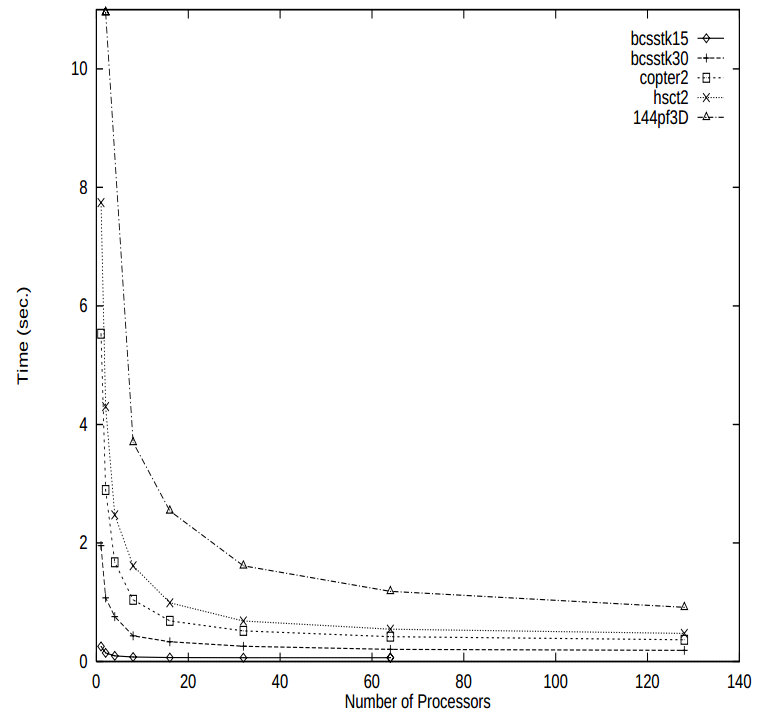
\includegraphics[width=0.5\textwidth]{figures/chapter-2/sparse-triangular-solve-performance.png}
\caption{Performance of sparse triangular solve \cite{sparse-la:triangular-solve}}
\label{fig:sparse-triangular-solve-performance}
\end{figure}


It is interesting to notice that performance of the triangular solver depends on a matrix sparsity structure as well as the matrix size. \\

Triangular solve \ref{eq:Gmres-5} can be computed in a single processor because matrix $R_m$ is usually small and depends on the number iterations before the restart. In this case the triangular solve can become a bottleneck again. \\


Figure \ref{fig:gmres-strong-scaling-speed-up} shows strong scaling performance results of the default GMRES solver from the PETSc library. The solver was set up without any preconditioner and 50 iterations as the restart. Additionally no stop criteria was specified except the maximum number iterations which was equal to 100. The \textit{spread} process pinning strategy, described in section \ref{subseq:matrix-sets-and-hardware}, was used. It is well-known that all iterative methods are memory bound due to indirect memory addressing caused by sparse matrix storage schemes. Hence equal process distribution can help reduce the load on memory channels since it is an obvious bottleneck for this type of applications. \\


Four matrices were chosen form the GRS matrix set for the tests, namely: cube-64, cube-645, k3-2 and k3-18. The information about the matrices is summarized in table \ref{table:grs-matrix-set}. As we expected, we can observe strong deviation of our results from the ideal speed-up line when the number of processes exceeds 10.\\


\figpointer{\ref{fig:gmres-strong-scaling-speed-up}}

It should be mentioned that parallelization overheads, introduced by such MPI operations as MPI\_Send, MPI\_Recv, MPI\_Allreduce, etc., also have their impact on performance of the algorithm.\\

Other Krylov methods such as CG, for example, scales much better than GMRES. Because of the nature of the CG algorithm the next search direction can be found using a recurrent expression and the algorithms boils down to simple operations such as dot products and matrix vector multiplications. These operations can be easily parallelized and drop of performance comes only from MPI overheads. A quite comprehensive study about parallel CG algorithm performance can be found in \cite{sparse-la:cg}. The authors also introduced a deeply pipelined version of CG algorithm that scales even better due to overlapping the time-consuming global communication phase, induced by parallel dot product computations, with useful independent computations \cite{sparse-la:cg}.\\


\figpointer{\ref{fig:gmres-strong-scaling-speed-up}}
\begin{figure}[htpb]
  \centering
  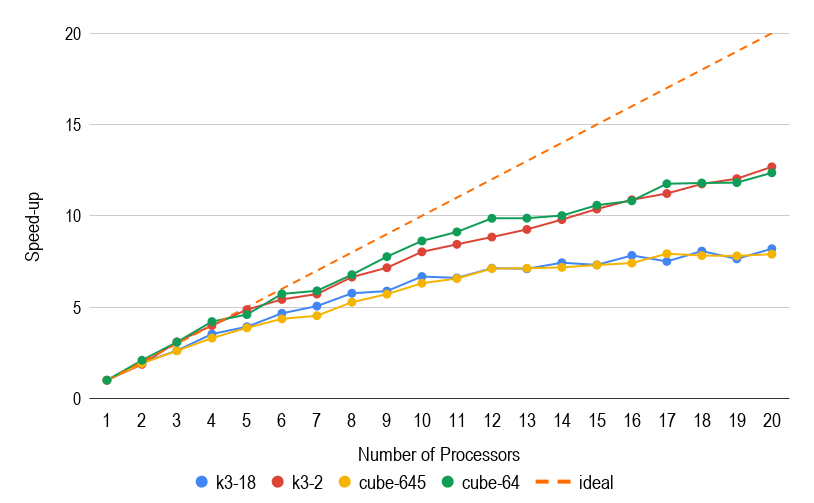
\includegraphics[width=0.7\textwidth]{figures/chapter-2/gmres-strong-scaling-speedup.png}
\caption{GMRES strong scaling speed-up}
\label{fig:gmres-strong-scaling-speed-up}
\end{figure}



% start discussion about preconditioning
The most important criteria of Krylov methods is convergence rate. The convergence rate of iterative methods strongly depends on a matrix and, in particular, on its condition number. For instance, equation \ref{eq:Gmres-7} shows dependence of the convergence rate from the matrix condition number. It can be clearly seen that a big condition number leads to very slow error reduction and, as the results, to huge number of iterations.\\

\begin{equation} \label{eq:Gmres-7}
	|| e^i ||_A \leq 2 ( \frac{\sqrt k - 1}{\sqrt k + 1} )^i || e^0 ||_A
\end{equation}

where $k = \frac{\lambda_{max}}{\lambda_{min}}$ - condition number of the corresponding matrix. \\

An obvious solution of such a problem is to reduce the condition number of the original system \ref{eq:slq}. A general method is to transform the original system in such a way that the conditional number of the transformed system gets significantly smaller. The transformation of \ref{eq:slq} can be done from the left side \ref{eq:pcn-1} or from the right one \ref{eq:pcn-2}.

\begin{equation} \label{eq:pcn-1}
	PAx = Pb
\end{equation}


\begin{equation} \label{eq:pcn-2}
	AP(P^{-1}x) = b
\end{equation}

where matrix $P$ is called preconditioner.\\


As an extreme example we can consider the inverse matrix $A^{-1}$ as the best preconditioner since it directly leads to the solution of the problem \ref{eq:slq} and, thus, it requires only one iteration. However, it is obvious that computation of inverse $A^{-1}$ is extremely expensive operation and it is not an objective of any iterative methods. That example helps understand and set requirements for preconditioners, namely:

\begin{enumerate}
	\item cheap to compute e.g. a 5-10 iterations of the corresponding Krylov solver
	\item should lead to a small conditioner number of the transposed system
	\item should be sparse, otherwise storage requirements will considerably increase
\end{enumerate}


There exist numerous techniques to compute preconditioners given a matrix $A$ e.g. (point) Jacobi, Block-Jacobi, incomplete $LU$ decomposition (ILU), multilevel ILU (ILU(p)), threshold ILU (ILUT), incomplete Cholesky factorization (IC), sparse approximate inverse (SPAI), multigrid as a preconditioner, etc. Almost all methods listed above have some tuning parameters which allow to get a better preconditioner i.e. a smaller condition number of the transformed system. However, it usually leads to increase of computational and storage costs. \\

Some methods can works particularly well for matrices derived from certain PDEs e.g. Poisson, Navier\-Stokes, etc. problems discretized using the cartesian grid. However sometimes it can take a considerable amount of time to choose correct parameters for a certain preconditioning algorithm. It can become a challenge to fulfill all requirements 1, 2, 3 mentioned above. \\

Table \todo{Table with comparisons of different preconditioning for our test cases}

Table [] shows results of different preconditioning algorithms applied to our test case. It can be seen that some algorithms failed even after tuning. \\

It interesting to notice that \citeauthor{wsmp} came to approximately the same results working on their set of matrices in their work \cite{wsmp}. They observed that preconditioned iterative solvers worked efficiently only for 2 out 5 cases in contrast to direct sparse solvers.\\

We can summarize that it is vital to perform careful parameter tuning of any preconditioning algorithms combining results from [table] and \cite{wsmp}. In general the  search can take a considerable amount of time. Moreover, it becomes impractical for time integration problems where topology of an underlying problem and, as the results, the computational mesh, discretization, Jacobian matrix can be changed over time of a simulation. It is obvious that parameters chosen for a particular time step can become not optimal for consecutive steps and, at the end, it can lead to divergence. If divergence happens at any time step the entire time integration algorithm fails and the simulation has to be restarted with different preconditioning parameters or with a different preconditioning algorithm.\\

By and large we come to a conclusion that preconditioned iterative solvers are not robust and thus cannot fully fulfill requirements listed in section \ref{chapter:solver configuration}.\\

% maybe above we have to mention inderect memory access and its effect on performance
